% This LaTeX was auto-generated from MATLAB code.
% To make changes, update the MATLAB code and export to LaTeX again.

\documentclass{article}

\usepackage[utf8]{inputenc}
\usepackage[T1]{fontenc}
\usepackage{lmodern}
\usepackage{graphicx}
\usepackage{color}
\usepackage{hyperref}
\usepackage{amsmath}
\usepackage{amsfonts}
\usepackage{epstopdf}
\usepackage[table]{xcolor}
\usepackage{matlab}

\sloppy
\epstopdfsetup{outdir=./}
\graphicspath{ {./Practica1_CarmenGallardo_PabloMendieta_images/} }

\matlabhastoc

\begin{document}

\label{T_47B18C65}
\matlabtitle{Práctica 1 - CARMEN GALLARDO Y PABLO MENDIE}

\matlabtableofcontents{ÍNDICE}
\label{H_CAA807EC}
\matlabheading{Definición de variables}

\begin{par}
\begin{flushleft}
Vamos a realizar el modelo de una supuesta propagación de una enfermedad. Definimos las siguientes variables:
\end{flushleft}
\end{par}

\begin{par}
$$\begin{array}{l}
\textrm{Pi}:\textrm{Nº}\;\textrm{de}\;\textrm{Personas}\;\textrm{infectadas}\\
\;\Pr :\textrm{Nº}\;\textrm{de}\;\textrm{Personas}\;\textrm{recuperadas}\\
\textrm{Población}:\textrm{Nº}\;\textrm{total}\;\textrm{de}\;\textrm{personas}\;\\
\textrm{Psuscep}:\textrm{Nº}\;\textrm{Personas}\;\textrm{suceptibles}\\
\textrm{TIC}:\textrm{Tasa}\;\textrm{de}\;\textrm{Infencción}\;\textrm{por}\;\textrm{Contacto}\to N\left(0\ldotp 4,0,1\right)\\
\textrm{TRI}:\textrm{Tasa}\;\textrm{de}\;\textrm{Recuperación}\;\textrm{de}\;\textrm{la}\;\textrm{Infección}\to \beta \left(4,1\right)
\end{array}$$
\end{par}

\begin{matlabcode}
clc, clear, clf
pi = 10;
pr = 0;
poblacion = 1000;
psuscept = poblacion - pi;
distTIC = [0.4 0.1];
distTRI = [4 1];
Fin = 25; %tiempo de parada
T = 1;
\end{matlabcode}

\label{H_56281233}
\matlabheading{Mecanismo de transición (Ecuaciones en difrencia)}

\begin{par}
\begin{flushleft}
Para obtener los mecanismos de transición que existen, vamos a tener en cuenta la variación de la población infectada y la variación de la población recuperada. 
\end{flushleft}
\end{par}

\begin{par}
\begin{flushleft}
Para calcular la variación de población infectada, tenemos que tener en cuenta la población susceptible de infectarse, es decir, la población total sin contar las personas ya infectadas y las que ya han pasado la infección Por otro lado hay que tener en cuenta las personas que se van a recuperar ese día. Para la variación de población recuperada simplemente hay que tener en cuenta las personas que están infectadas. Las ecuaciones quedarían de la siguiente manera:
\end{flushleft}
\end{par}

\begin{par}
$$\Delta p_i =\textrm{TIC}*\left(\textrm{población}-\left(p_i -p_r \right)\right)-\textrm{TRI}*p_i$$
\end{par}

\begin{par}
$$\Delta \textrm{pr}=\textrm{TRI}*p_i$$
\end{par}

\begin{par}
\begin{flushleft}
Sabemos tambien lo siguiente:
\end{flushleft}
\end{par}

\begin{par}
$$p_{\textrm{suscep}} =\;$$$$\left(\textrm{población}-\left(p_i -p_r \right)\right)$$
\end{par}

\begin{par}
\begin{flushleft}
Ahora, para obtener las ecuaciones en diferencia sustituimos la variación de la siguiente manera:
\end{flushleft}
\end{par}

\begin{par}
$$\Delta p_i =\frac{{\textrm{pi}}_{n+1} -{\textrm{pi}}_n }{\Delta t}$$
\end{par}

\begin{par}
$$\Delta p_i =\frac{{\textrm{pr}}_{n+1} -{\textrm{pr}}_n }{\Delta t}$$
\end{par}

\begin{par}
\begin{flushleft}
Suponemos que $\Delta t$ es igual a 1, porque queremos analizar el modelo día a día. De esta manera nos quedan las siguientes ecuaciones en difrencia: 
\end{flushleft}
\end{par}

\begin{par}
$${\textrm{pi}}_{n+1} =\textrm{TIC}*{\textrm{psuscep}}_n -\textrm{TRI}*{\textrm{pi}}_n +{\textrm{pi}}_n$$
\end{par}

\begin{par}
$${\textrm{pr}}_{n+1} =\textrm{TRI}*{\textrm{pi}}_n +{\textrm{pr}}_n$$
\end{par}

\begin{par}
$${\textrm{psucept}}_{n+1} ={\textrm{psuscep}}_n -{\textrm{pi}}_n -{\textrm{pr}}_n$$
\end{par}

\label{H_EEE2C88F}
\matlabheading{Diagrama de Flujo}

\begin{par}
\begin{flushleft}
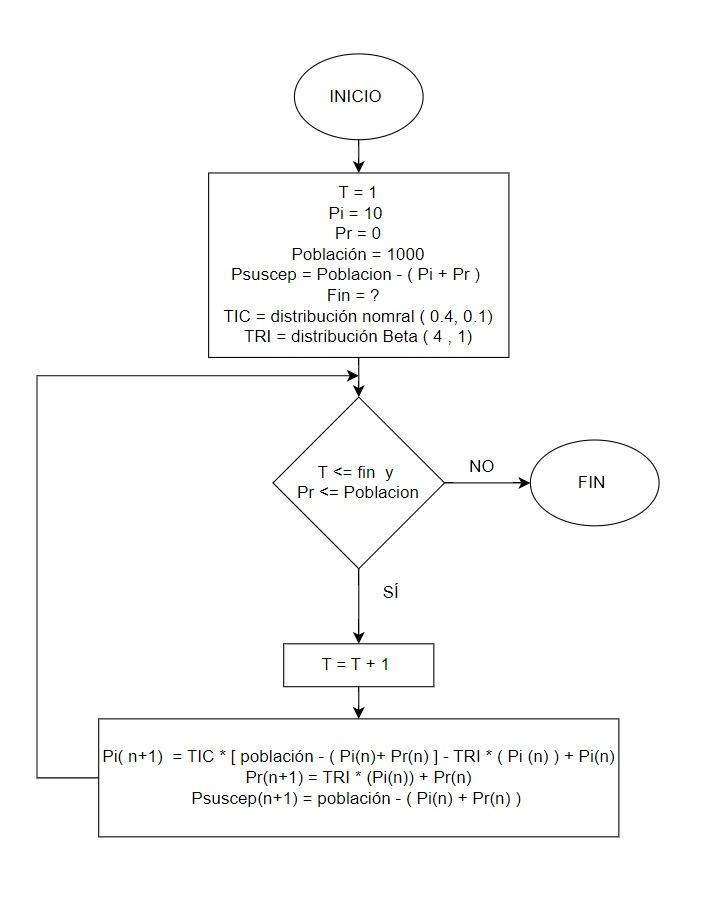
\includegraphics[width=\maxwidth{41.04365278474661em}]{image_0}
\end{flushleft}
\end{par}

\label{H_99016AE3}
\matlabheading{Traza}

\begin{par}
\begin{flushleft}
Para analizar que el diagrama de flujo es correcto, realizamos la traza con excel (suponemos que TIC y TRI son 0.4 y 0.8 respectivamente):
\end{flushleft}
\end{par}

\begin{par}
\begin{flushleft}
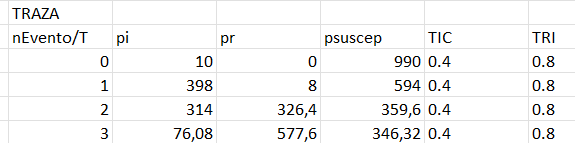
\includegraphics[width=\maxwidth{57.7019568489714em}]{image_1}
\end{flushleft}
\end{par}

\begin{par}
\begin{flushleft}
Observamos que dan valores con sentido.
\end{flushleft}
\end{par}


\label{H_83D80EF5}
\matlabheading{Solución gráfica}

\begin{par}
\begin{flushleft}
Para calcular la solución grafica utilizamos una función qeu replica el diagram de flujo
\end{flushleft}
\end{par}

\begin{matlabcode}
[vectorpi, vectorpr,vectorsuscep] = infeccion (T, Fin,poblacion,psuscept,pi,pr, distTIC, distTRI );
plot(T-1:Fin,vectorpi, '-*r')
hold on
plot(T-1:Fin,vectorpr, '-*b')
hold on
plot(T-1:Fin,vectorsuscep, '-*', 'Color',[0.2,0.6,0.2])
xlabel("Tiempo (días)")
ylabel("Población")
title("Modelo epidemológico")
legend('Infectados', 'Recuperados','Susceptibles', 'Location', 'east')
grid on
hold off
\end{matlabcode}
\begin{center}
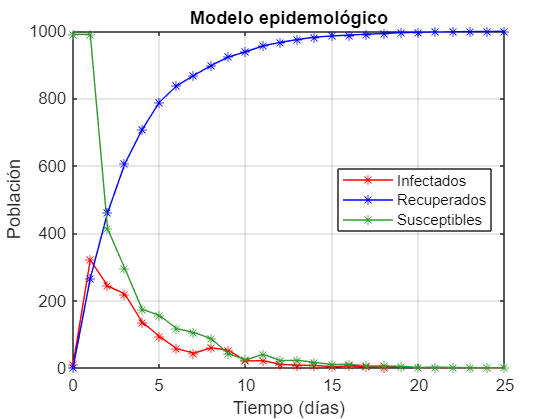
\includegraphics[width=\maxwidth{44.7566482689413em}]{figure_0.png}
\end{center}

\begin{par}
\begin{flushleft}
Al observar la gráfica vemos que el sistema tiende a la estabilidad, donde la población de recuperados  tiende a la población total y el número de infectados tiende a cero. Esto tiene sentdio ya que la toda la población acabará pasando la infección.
\end{flushleft}
\end{par}



\vspace{1em}
\begin{matlabcode}
function [vectorpi, vectorpr, vectorsuscep] = infeccion (T, Fin,poblacion,psuscep,pi,pr, distTIC, distTRI )
    
    vectorpi = pi;
    vectorpr = pr;
    vectorsuscep = psuscep;
    %Rutina de parada
    while T<= Fin && pr<=poblacion 
        %Rutina de tiempo
        T = T + 1;
        
        %Rutina de evento
        TIC = normrnd(distTIC(1),distTIC(2)); %al randomizar estos datos pueden dar valores negativos lo cual genera infectados negativos (afecta tambien a susceptibles)
        TRI = betarnd(distTRI(1),distTRI(2));
        psuscep = poblacion- pi  - pr;
        pi = TIC*(psuscep) - TRI*pi + pi; 
        pr = TRI*pi + pr;
        

        vectorpi = [vectorpi pi];
        vectorpr = [vectorpr pr];
        vectorsuscep = [vectorsuscep psuscep];
    end    
end
\end{matlabcode}

\end{document}
